\chapter{Resultados}


\begin{figure}[H]
    \centering
    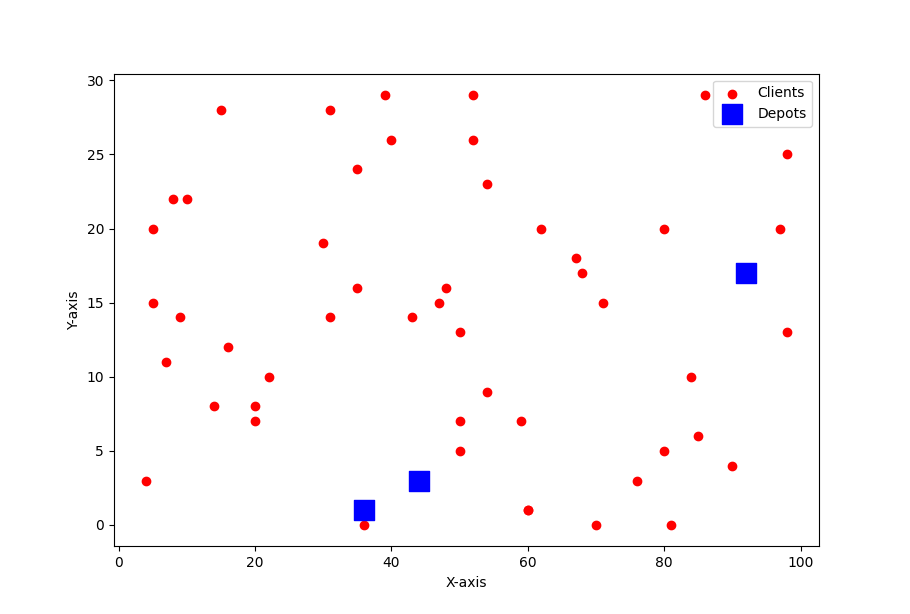
\includegraphics[width=\linewidth]{img/inst_1.png}
    \caption{Instância do problema}
    \label{fig:inst1}
  \end{figure}
  
  \subsection*{Estrutura de dados}
  \label{subsec:estruturadosdados}
  \textcolor{red}{A principal estrutura de dados utilizada nas heurísticas e nos modelos é dedicada à representação das plantas, onde podemos acessar em cada instante as viagens que são realizadas. Mais profundamente, corresponde a um vetor de tamanho igual ao horizonte de tempo, onde cada posição desse vetor armazenará as viagens que ocorrerão em cada um dos seus instantes. Por exemplo, caso a viagem 3 seja executada no período de 10 a 20, adicionaremos o valor 3 nas posições [10,20) do vetor. A quantidade de viagens em cada instante representa a quantidade mínima de veículos utilizadas por essa planta nesse instante. A maior quantidade de viagens simultâneas representará a quantidade de veículos utilizados pela planta. 
  Na imagem abaixo, vemos uma representação dessa estrutura de dados utilizada.}
  
  % \captionsetup{aboveskip=0pt,belowskip=1pt}
  \begin{figure}[H] % "H" ensures the figure stays in the exact place
    \centering
    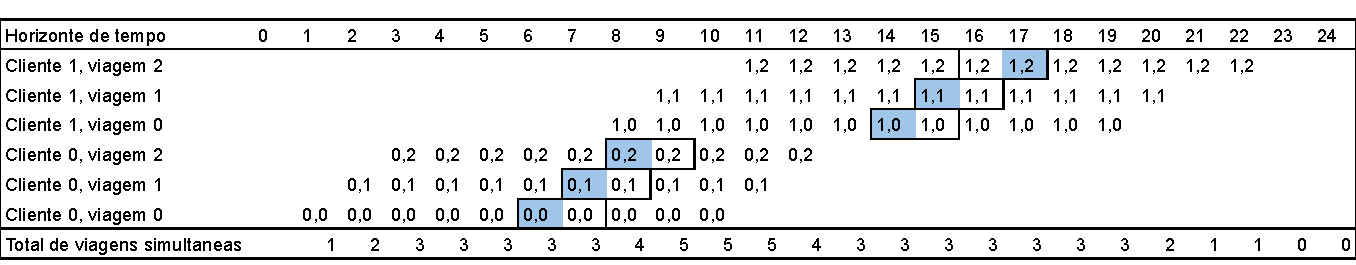
\includegraphics[width=1\textwidth]{img/estrutura de dados.pdf}
    \caption{Estrutura de Dados}
  \end{figure}
  
   \textcolor{red}{No exemplo da figura acima, temos a atribuição das viagens de dois clientes a uma planta. A janela de tempo para entrega é de duas unidades de tempo e estão com bordas nos instantes cuja entregas são permitidas. As viagens do cliente 0 custam 4 unidades de tempo para a ida e 4 unidades de tempo para a volta, enquanto as viagens do cliente 1 custam 6 unidades de tempo em cada sentido. Os instantes em azul indicam o momento das entregas.
  Nesse exemplo, a viagem 2 do cliente 1 foi executada no último instante da janela de tempo, fazendo assim com que a quantidade de viagens simultâneas no instante 10 não chegasse a seis, fazendo com que a necessidade de veículos nessa planta não superasse 5 em nenhum instante. }
  